\documentclass[10pt,twocolumn]{article}

\usepackage[margin=0.72in]{geometry}
\usepackage{amsmath,amssymb,bm}
\usepackage{booktabs}
\usepackage{graphicx}
\usepackage{microtype}
\usepackage{xcolor}
\usepackage{hyperref}
\usepackage{tikz}
\usetikzlibrary{arrows.meta,positioning,fit,calc}

\hypersetup{colorlinks=true,allcolors=blue!55!black}
\newcommand{\SE}{\mathrm{SE}(3)}
\newcommand{\SO}{\mathrm{SO}(3)}
\newcommand{\Exp}{\operatorname{Exp}}
\newcommand{\Log}{\operatorname{Log}}
\newcommand{\R}{\mathbb{R}}

\title{Temporally Consistent RGB--CAD Recovery and Learned $\SE$ Filtering for Long-Range Vehicle Pose Tracking}
\author{Anonymous Authors\\
\small Draft methods section for integration into a larger paper}
\date{}

\begin{document}
\maketitle

\begin{abstract}
Per-frame category-level and novel-object pose estimators can produce accurate
measurements under favorable viewing conditions, but their trajectories may
contain depth outliers, abrupt translation changes, and approximately
$180^\circ$ front--rear orientation flips. We present a causal, sequence-aware
post-processing pipeline for single-vehicle six-degree-of-freedom pose
tracking. The method first expands each GigaPose estimate into RGB--CAD pose
hypotheses, uses a gated recurrent unit (GRU) to select candidates over time,
and resolves ambiguous orientation transitions with confidence-adaptive
hysteresis and fixed-lag backfilling. A second learned error-state filter then
predicts diagonal Kalman-style gains on $\SE$ to smooth translation alone or
the full pose. The design separates discrete hypothesis recovery from
continuous motion filtering, resets all temporal state at sequence
discontinuities, and retains measurement-relative safety fallbacks. On a
328-frame development-validation set containing distinct front- and
rear-camera sequences, the fixed-lag selector reduced median translation and
rotation error from 3.07~m and $15.50^\circ$ to 0.66~m and $5.46^\circ$,
respectively. A translation-only learned filter further reduced median
translation error to 0.59~m while preserving the selector orientation exactly.
These numbers are development-validation results; final claims should use the
separate unseen benchmark described in Sec.~\ref{sec:protocol}.
\end{abstract}

\section{Method}
\label{sec:method}

\subsection{Problem formulation}

For a monocular RGB sequence $\{I_t\}_{t=1}^{T}$, camera intrinsics $K_t$, an
object mask or detection $M_t$, and a CAD model $\mathcal{C}$, the objective is
to estimate the camera-to-object pose
\begin{equation}
    T_t = T_{\mathrm{camera},\mathrm{object},t}
    = \begin{bmatrix}R_t & \bm{p}_t\\ \bm{0}^{\top} & 1\end{bmatrix}
    \in \SE,
\end{equation}
where $R_t\in\SO$ and $\bm{p}_t\in\R^3$. GigaPose
\cite{nguyen2024gigapose} provides one or more per-frame measurements
$\{T^{\mathrm{GP}}_{t,k}\}$. Although these estimates contain useful
appearance and geometric evidence, per-frame inference does not enforce
trajectory consistency. Our goal is therefore to recover a temporally
coherent pose without requiring depth, LiDAR, or a map at inference time.

We assume one target vehicle per sequence. Consequently, the present method
does not solve multi-object association; its temporal state is reset whenever
the source run, camera, or continuous frame segment changes.

\begin{figure*}[t]
\centering
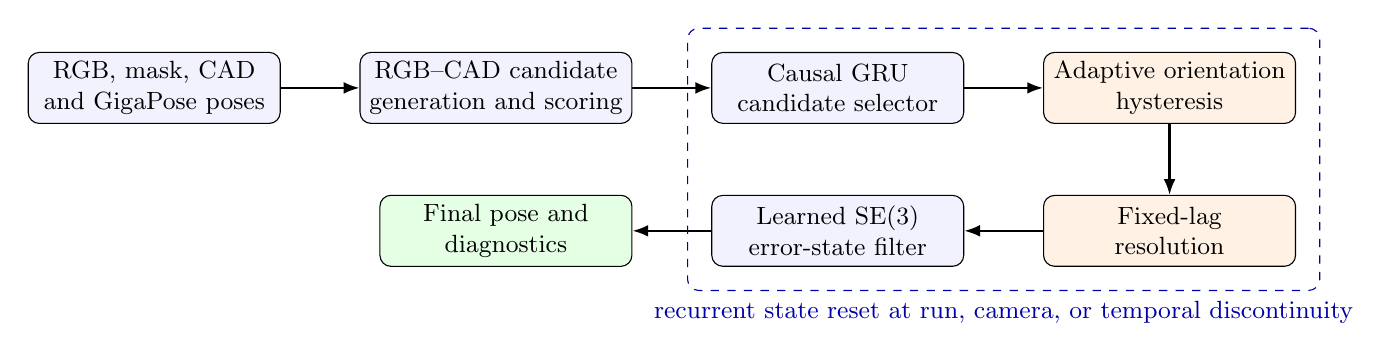
\begin{tikzpicture}[
  node distance=9mm and 10mm,
  block/.style={draw,rounded corners,align=center,minimum height=9mm,
                minimum width=32mm,fill=blue!5,font=\small},
  decision/.style={draw,rounded corners,align=center,minimum height=9mm,
                   minimum width=32mm,fill=orange!10,font=\small},
  output/.style={draw,rounded corners,align=center,minimum height=9mm,
                 minimum width=32mm,fill=green!10,font=\small},
  arrow/.style={-{Latex[length=2mm]},thick}
]
\node[block] (input) {RGB, mask, CAD\\and GigaPose poses};
\node[block,right=of input] (cand) {RGB--CAD candidate\\generation and scoring};
\node[block,right=of cand] (gru) {Causal GRU\\candidate selector};
\node[decision,right=of gru] (orient) {Adaptive orientation\\hysteresis};
\node[decision,below=of orient] (lag) {Fixed-lag\\resolution};
\node[block,left=of lag] (kf) {Learned $\SE$\\error-state filter};
\node[output,left=of kf] (out) {Final pose and\\diagnostics};
\draw[arrow] (input)--(cand);
\draw[arrow] (cand)--(gru);
\draw[arrow] (gru)--(orient);
\draw[arrow] (orient)--(lag);
\draw[arrow] (lag)--(kf);
\draw[arrow] (kf)--(out);
\node[draw=blue!65!black,dashed,rounded corners,fit=(gru)(orient)(lag)(kf),
      inner sep=3mm,label={[blue!65!black,font=\small]below:
      recurrent state reset at run, camera, or temporal discontinuity}] {};
\end{tikzpicture}
\caption{Inference pipeline. The candidate selector addresses multimodal and
discrete pose ambiguity, especially front--rear flips. The learned error-state
filter subsequently performs continuous translation or full-pose smoothing.
Adaptive orientation and fixed-lag decisions occur before the learned filter.}
\label{fig:pipeline}
\end{figure*}

\subsection{RGB--CAD hypothesis generation}

For each frame, we construct a bounded candidate set
$\mathcal{H}_t=\{T_{t,j}\}_{j=1}^{N}$ around the top GigaPose hypotheses. The
set includes translation/depth offsets, image-center offsets, local rotation
perturbations, explicit yaw perturbations, and an approximately $180^\circ$
orientation alternative. A matching network combines spatial RGB/mask
features, rendered CAD features, and frozen DINOv2 patch features
\cite{oquab2023dinov2}. Each hypothesis is represented by a feature vector
\begin{equation}
\begin{aligned}
\bm{c}_{t,j} = [&q_{t,j},s_{t,j},\mathrm{IoU}_{t,j},
\Delta u_{t,j},\Delta\log z_{t,j},\\
&\Delta R_{t,j},\Delta T^{\mathrm{GP}}_{t,j},
\bm{r}^{6\mathrm{D}}_{t,j},\bm{b}_{t,j}],
\end{aligned}
\end{equation}
where $q$ is confidence, $s$ is the learned RGB--CAD quality score,
$\mathrm{IoU}$ measures rendered-mask agreement, $\bm{r}^{6\mathrm{D}}$ is a
continuous rotation representation, and $\bm{b}$ encodes the proposal type.

The candidate exporter intentionally assigns zero weight to its legacy
history term. This prevents a hand-designed temporal score from eliminating a
valid recovery hypothesis before the learned sequence model observes it. All
temporal selection is delegated to the GRU and orientation resolver.

\subsection{Causal GRU candidate selection}

Let $\bm{f}_t$ denote frame-level measurement and detection context. A causal
GRU updates its hidden state and predicts a logit for each candidate:
\begin{align}
\bm{h}_t &= \mathrm{GRU}(\{\bm{c}_{t,j}\}_{j=1}^{N},\bm{f}_t,\bm{h}_{t-1}),\\
\ell_{t,j} &= g_{\theta}(\bm{c}_{t,j},\bm{f}_t,\bm{h}_t),\\
\pi_{t,j} &= \frac{\exp(\ell_{t,j})}{\sum_k\exp(\ell_{t,k})}.
\end{align}
The selector is trained with cross-entropy against the candidate having the
lowest normalized pose error. Translation and geodesic rotation errors are
combined only to construct this oracle candidate label; ground truth is not
used during inference.

Because a selector cannot choose a pose that is absent from $\mathcal{H}_t$,
the proposal set includes orientations based on the previous accepted pose and
constant angular velocity, in addition to perturbations of the current
GigaPose pose. This is essential when the current per-frame estimate is already
front--rear flipped.

\subsection{Adaptive orientation hysteresis}
\label{sec:hysteresis}

The temporal orientation prediction is
\begin{equation}
\widehat{R}_{t}^{-}=R_{t-1}\Exp(\bm{\omega}_{t-1}\Delta t),
\end{equation}
and candidate $j$ is compared to it with the geodesic distance
\begin{equation}
\theta_{t,j}=
\left\|\Log\left((\widehat{R}_{t}^{-})^{\top}R_{t,j}\right)\right\|_2.
\end{equation}
Candidates below $45^\circ$ receive no additional penalty; candidates between
$45^\circ$ and $90^\circ$ receive a soft rotation-jump penalty. Changes above
$135^\circ$ are treated as transitions between persistent front--rear modes,
rather than ordinary orientation updates.

Let $m_t\in\{0,1\}$ denote the persistent orientation mode. A proposed mode
change opens a pending interval. The required confirmation length adapts to
the stability of the current mode:
\begin{equation}
n_{\mathrm{confirm}} =
\begin{cases}
2, & n_{\mathrm{stable}}<4,\\
5, & n_{\mathrm{stable}}\geq4.
\end{cases}
\end{equation}
Pending observations must be mutually consistent within $45^\circ$ and meet
minimum selector probability and margin requirements. A normal candidate
consistent with the established mode cancels the pending transition. Thus, an
isolated high-confidence error cannot immediately reverse a stable track.

\subsection{Fixed-lag orientation resolution}

Causal hysteresis alone protects the current output by retaining its temporal
orientation during an unresolved transition. If the transition later proves
genuine, however, those earlier frames would remain assigned to the old mode.
We therefore buffer the pending interval. Once the evidence confirms a mode
change, the resolver backfills the interval with the selected orientations in
the confirmed mode. If the transition is rejected, the buffered interval is
committed in the previous mode. The maximum delay equals the adaptive
confirmation horizon (two or five frames in our implementation).

This operation is a fixed-lag smoother only for the discrete orientation mode;
it does not use future information beyond the bounded pending interval and
does not alter translation.

\subsection{Learned $\SE$ error-state filtering}

After fixed-lag resolution, a KalmanNet-style recurrent filter
\cite{revach2022kalmannet} performs continuous smoothing. Its state is
\begin{equation}
\bm{x}_t=(\bm{p}_t,R_t,\bm{v}_t,\bm{\omega}_t),
\end{equation}
with constant linear- and angular-velocity prediction
\begin{align}
\widehat{\bm{p}}_t^- &= \bm{p}_{t-1}+\bm{v}_{t-1}\Delta t,\\
\widehat{R}_t^- &= R_{t-1}\Exp(\bm{\omega}_{t-1}\Delta t).
\end{align}
Given measurement $(\bm{p}_t^m,R_t^m)$, the innovations are
\begin{align}
\bm{e}_t^p &= \bm{p}_t^m-\widehat{\bm{p}}_t^-,\\
\bm{e}_t^R &= \Log\left((\widehat{R}_t^-)^{\top}R_t^m\right).
\end{align}
The recurrent input concatenates normalized innovations, the previous linear
and angular velocities, $\Delta t$, and measurement context
\begin{equation}
\bm{u}_t=[\bm{e}_t^p,\bm{e}_t^R,\bm{v}_{t-1},\bm{\omega}_{t-1},
\Delta t,\bm{d}_t],
\end{equation}
where $\bm{d}_t$ contains measurement confidence, normalized bounding-box
center, width, height, area, and measured depth. A GRU predicts 12 diagonal
gains in $(0,1)$:
\begin{equation}
[\bm{k}_t^p,\bm{k}_t^R,\bm{k}_t^v,\bm{k}_t^{\omega}]
=\sigma(g_{\phi}(\mathrm{GRU}(\bm{u}_t))).
\end{equation}
The update is
\begin{align}
\bm{p}_t &= \widehat{\bm{p}}_t^-+\bm{k}_t^p\odot\bm{e}_t^p,\\
R_t &= \widehat{R}_t^-\Exp(\bm{k}_t^R\odot\bm{e}_t^R),\\
\bm{v}_t &= \bm{v}_{t-1}+\bm{k}_t^v\odot\bm{e}_t^p/\Delta t,\\
\bm{\omega}_t &= \bm{\omega}_{t-1}
 +\bm{k}_t^{\omega}\odot\bm{e}_t^R/\Delta t.
\end{align}
Unlike a classical Kalman filter, the method does not explicitly propagate
covariance matrices $P$, $Q$, and $R$. The learned gains approximate an
adaptive correction policy while the explicit $\SE$ prediction preserves the
state-space structure.

We train two variants. The \emph{translation-only} model applies the learned
translation update but copies the fixed-lag selector rotation exactly:
\begin{equation}
R_t^{\mathrm{out}}=R_t^m.
\end{equation}
The \emph{full-pose} model applies both learned translation and rotation
updates. At inference, corrections exceeding configured translation or
rotation limits are rejected in favor of the input measurement.

\subsection{Filter training objective}

For valid frames after the first element of each clip, the full-pose filter is
trained using
\begin{equation}
\mathcal{L}_{\mathrm{pose}}=
\frac{\|\bm{p}_t-\bm{p}_t^{*}\|_2}{s_p}
+\frac{d_{\SO}(R_t,R_t^{*})}{s_R},
\end{equation}
where
\begin{equation}
d_{\SO}(R_1,R_2)=
\left\|\Log(R_1^{\top}R_2)\right\|_2.
\end{equation}
A weak measurement-preservation regularizer discourages unnecessary changes:
\begin{equation}
\mathcal{L}=\mathcal{L}_{\mathrm{pose}}+lambda_{\mathrm{pres}}
\left(
\frac{\|\bm{p}_t-\bm{p}_t^m\|_2}{s_p}+
\frac{d_{\SO}(R_t,R_t^m)}{s_R}
\right).
\end{equation}
For the translation-only model, both rotation terms are omitted and the input
rotation is preserved by construction. Models are trained on consecutive
clips; clips never cross run, camera, or discontinuity boundaries.

\subsection{Relation to GRUTrack}

The proposed filter shares the learned-gain motivation of KalmanNet and the
open-source GRUTrack system \cite{grutrack2025}. GRUTrack is a complete
nuScenes multi-object tracker that combines learned Kalman gains with data
association, track lifecycle management, and automotive box states such as
position, dimensions, planar velocity, acceleration, yaw, and yaw rate. In
contrast, our model assumes one already-associated vehicle, operates directly
on camera-to-object poses in $\SE$, and estimates full three-dimensional
rotation and angular velocity. The RGB--CAD candidate selector and fixed-lag
front--rear state are also specific to our formulation. Accordingly, the
implementation should be viewed as a task-specific KalmanNet-style filter,
not as a reproduction of GRUTrack.

\section{Experimental Protocol}
\label{sec:protocol}

\paragraph{Data separation.}
Assetto Corsa sequences are partitioned by physical source run, not by random
frame. Consecutive clips from one run therefore cannot appear in both training
and evaluation. Front and rear cameras are represented separately, and all
recurrent state is reset when the source run, camera, frame continuity, or
timestamp continuity changes. A final benchmark contains 5,174 usable frames
from four unseen sequences after excluding 361 manifest rows without an
unambiguous joined 3D box/instance-mask identifier. It covers distances from
0--140~m. Since training used samples only through 120~m, the 120--140~m bin
must be reported separately as out-of-distribution.

\paragraph{Metrics.}
Translation error and geodesic rotation error are
\begin{align}
e_t &= \|\bm{p}_t-\bm{p}_t^*\|_2,\\
e_R &= \frac{180}{\pi}
\cos^{-1}\!\left(\mathrm{clip}\left(
\frac{\mathrm{tr}(R_t^{\top}R_t^*)-1}{2},-1,1\right)\right).
\end{align}
We report mean, median, and 90th percentile errors; recall below 1~m and
$10^\circ$; per-distance-bin performance; and paired frame-level improvement
fractions relative to GigaPose. Front and rear cameras should additionally be
reported separately.

\paragraph{Required ablations.}
The final comparison should include: (i) GigaPose; (ii) standalone RGB
self-recovery; (iii) GRU candidate selection without adaptive orientation;
(iv) adaptive orientation without fixed lag; (v) the complete fixed-lag
selector; (vi) a GRU--Kalman filter applied directly to raw GigaPose; and
(vii) fixed-lag selector followed by translation-only or full-pose learned
filtering. Candidate generation and evaluation frames must be identical across
these conditions.

\section{Development-Validation Results}
\label{sec:results}

Table~\ref{tab:development} summarizes the currently available 328-frame
development-validation result containing Laguna front and Putnam rear
sequences. Checkpoints were selected using this development regime; therefore,
these values demonstrate pipeline behavior but must not be presented as final
unseen-test performance.

\begin{table*}[t]
\centering
\caption{Development-validation results on 328 frames. Lower error is better;
higher recall is better. ``T-only'' preserves fixed-lag rotation exactly.}
\label{tab:development}
\begin{tabular}{lrrrrrr}
\toprule
Method & Med. $e_t$ (m) & P90 $e_t$ (m) & Med. $e_R$ ($^\circ$) &
P90 $e_R$ ($^\circ$) & $e_t\!\leq\!1$m & $e_R\!\leq\!10^\circ$ \\
\midrule
GigaPose & 3.072 & 17.786 & 15.496 & 163.026 & 10.98\% & 41.16\% \\
GRU selector + adaptive fixed lag & 0.662 & 7.697 & 5.464 & 23.035 & 58.84\% & 70.43\% \\
+ learned filter (T-only) & 0.594 & \textbf{5.540} & 5.464 & \textbf{23.035} & 61.89\% & \textbf{70.43\%} \\
+ learned filter (full pose) & \textbf{0.592} & 6.057 & \textbf{4.728} & 23.238 & \textbf{62.20\%} & 69.51\% \\
\bottomrule
\end{tabular}
\end{table*}

Relative to GigaPose, the fixed-lag selector improved translation on 85.1\%
of paired frames and rotation on 67.4\%. The translation-only cascade improved
translation on 88.1\% of frames while retaining the same orientation as the
selector. Full-pose filtering improved rotation on 77.4\% of paired frames,
but its $10^\circ$ recall was slightly lower than that of the selector. This
trade-off motivates reporting both cascade variants rather than selecting one
solely from an aggregate loss.

\section{Limitations and Scope}

The current formulation assumes one known CAD object and does not perform
multi-object data association. The learned filter cannot create a correct
hypothesis when every upstream candidate is wrong; recovery from catastrophic
measurements is primarily the responsibility of candidate generation and the
selector. Fixed-lag hysteresis adds a bounded output delay. Its thresholds are
currently fixed hyperparameters and may require calibration under different
frame rates. The simulator-to-real gap remains a central risk: appearance,
mask quality, motion statistics, camera calibration, and GigaPose error modes
can all shift. Finally, the reported development-validation values should not
be interpreted as final generalization estimates. The unseen 5,174-frame
benchmark and a real-world sequence evaluation are required before making
conclusive performance claims.

\paragraph{Reproducibility note.}
For every experiment, the paper should record the GigaPose checkpoint, RGB--CAD
checkpoint, GRU selector checkpoint, learned-filter checkpoint, candidate
configuration, sequence-gap thresholds, orientation-hysteresis thresholds,
fixed-lag setting, correction guards, translation units, CAD origin, camera
split, and exact physical run identifiers.

\bibliographystyle{plain}
\bibliography{references}

\end{document}
